\section{Finding 6 - Weak password for User Bluey}
%center under chapter title a one row table with 6 coloumns and no borders
\vspace*{-0,3cm}
\begin{center}
    \begin{tabular}{c c c c}
        \textbf{Classification:} & Weak Password & \textbf{Severity:} & \textbf{\textcolor{red}{High}}  
        \end{tabular}
\end{center}

\vspace*{-0,7cm}
\begin{center}
    \begin{tabular}{c c}
        \textbf{CVE:} & CVE-2022-1039
    \end{tabular}
\end{center}

Using the Tool ”Hydra” the Password for the User ”bluey” was found in a very short amount of time with Brute Force. The Password is ”phoenix”. As a passwordlist the file ”rockyou.txt” was used which contains about 14 million common passwords. This file can be found online and is accessible for everyone.

\subsection{Finding Impact}
With the password it is possible to login to the \ac{DUT} as the User ”bluey” via ssh. This allows attackers to gain access to the \ac{DUT} and to execute commands as the User ”bluey”. This could lead for example to a 
\ac{RCE} or to a privlige escaltion (horizontal or vertical).

\subsection{Finding Details}
The Password was found using the Tool ”Hydra” with the following command:
\begin{lstlisting}[language=bash]
$ hydra -l bluey -P rockyou.txt 172.16.0.29 ssh -t 4 -V -I
\end{lstlisting}

After the password was found it was possible to login to the \ac{DUT} as the User ”bluey” via ssh:
%image here
\begin{figure}[h]
    \centering
    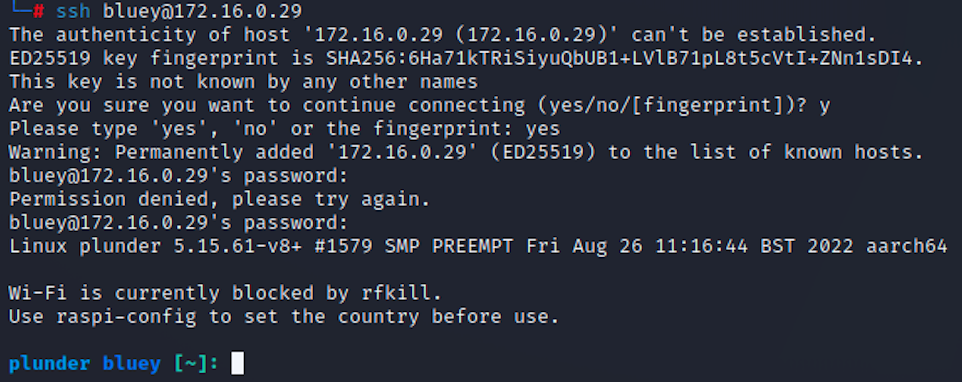
\includegraphics[width=0.8\textwidth]{img/ssh-access-bluey.png}
    \caption{Login as User Bluey}
    \label{fig:fin6}
\end{figure}


\subsection{Evaluation of Results}
\begin{center}
    \begin{tabular}{cccc}
    \textbf{Effort to Fix:} & &\ \textbf{\textcolor{green!50!blue}{Low}}\
    \end{tabular}
\end{center}
The password should be changed immediately. Notice that passwordlength is the most important aspect. Don't use common passwords.
